\documentclass[border=8pt]{standalone}
\usepackage{tikz}
\usetikzlibrary{arrows.meta,positioning,calc,fit}
\begin{document}
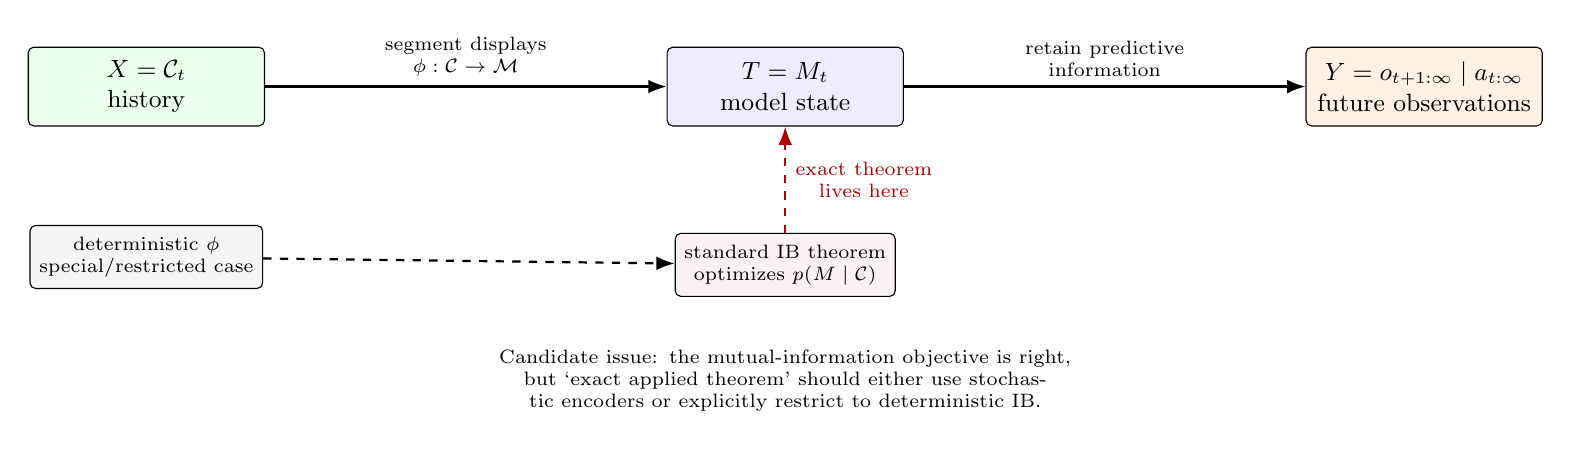
\begin{tikzpicture}[
  box/.style={draw, rounded corners=2pt, align=center, minimum width=3.0cm, minimum height=1.0cm, font=\small},
  small/.style={draw, rounded corners=2pt, align=center, minimum width=2.7cm, minimum height=0.8cm, font=\scriptsize},
  arr/.style={-Latex, thick},
  note/.style={align=center, font=\scriptsize}
]

\node[box, fill=green!7] (C) {$X=\mathcal C_t$\\history};
\node[box, fill=blue!7, right=5.1cm of C] (M) {$T=M_t$\\model state};
\node[box, fill=orange!10, right=5.1cm of M] (Y) {$Y=o_{t+1:\infty}\mid a_{t:\infty}$\\future observations};

\draw[arr] (C) -- node[above, note] {segment displays\\$\phi:\mathcal C\to\mathcal M$} (M);
\draw[arr] (M) -- node[above, note] {retain predictive\\information} (Y);

\node[small, below=1.35cm of M, fill=purple!6] (kernel) {standard IB theorem\\optimizes $p(M\mid\mathcal C)$};
\draw[arr, dashed, red!70!black] (kernel) -- node[right, note] {exact theorem\\lives here} (M);

\node[small, below=1.25cm of C, fill=gray!8] (det) {deterministic $\phi$\\special/restricted case};
\draw[arr, dashed] (det) -- (kernel);

\node[note, below=0.55cm of kernel, text width=8.0cm] {Candidate issue: the mutual-information objective is right, but `exact applied theorem' should either use stochastic encoders or explicitly restrict to deterministic IB.};

\end{tikzpicture}
\end{document}
